Several mechanisms have been identified to explain the evolution of cooperation among non-kin \citep{Trivers1971, MaynardSmith1974, Axelrod1981}, including positive reciprocity \cite{Trivers1971, Axelrod1981, Andre2007}, punishment \cite{Bshary2005, Raihani2012} or partner choice \cite{Eshel1982, Bull1991, West2007, Schino2017}. Among these mechanisms, partner choice has been considered over the last twenty years as having probably played a particularly important role \cite{Baumard2013a, +ref}. When individuals can choose among several different partners, which they can compare and compete against each other as in an economic market, this generates a selection pressure to cooperate more, to appear as a good partner and attract others' cooperation \cite{Noe1994}.

The effects of partner choice have been well documented in a large number of biological systems. For example, in the interaction between cleaner fishes and their clients the law of supply and demand determines the way in which the added value of the interaction is shared, in accordance with market principles \cite{Bshary2006}. When cleaners are rare, clients tolerate cheating on their part, while they become more picky when cleaners are numerous. The effects of partner choice have also been documented in primate grooming behavior in two meta-analyses, showing that female primates groom preferentially those that groom them most and that a positive relation exists between grooming and agonistic support \citep{Schino2007, Schino2008}. In vervet monkeys, individuals groom others in exchange for access to food and they do so for longer periods when fewer partners are available \cite{Fruteau2009}. Beyond cooperation, partner choice also plays a decisive role in mating, leading to the evolution of secondary sexual caracteristics and nuptial gifts, and/or to assortative matching (refs xxxTODOxxx \cite{Zahavi1975, xxTerrain}. Lastly, the effects of partner choice have also been documented in humans where it has been shown that the need to attract social partners is a major driver of cooperation \citep{Barclay2007a, Barclay2015, Barclay2016, Debove2015b,  Andre2011, Baumard2013a}.

% xx \cite{Clutton-brock2009} qui discute plein de cas de réciprocité qui pourrait n'être qu'en fait manipulations et mutualismes


There are, however, a number of biological situations in which one would typically expect partner choice to play an important role, but where no such effect has ever been demonstrated. These include most intraspecific collective actions in non-human animals. This is particularly salient in collective hunts such as collobus hunting in chimpanzees, or pack hunting in carnivores. No empirical evidence in these species suggests that individuals cooperate for reasons related to partner choice, either to attract partners or to be accepted by them in their hunts. On the contrary, the majority of available data are consistent with the more parcimonious explanation that individuals are simply doing what is in their immediate best interest at any given time \cite{Packer1986,Packer1988a, Melis2008, Melis2011}. In particular, if cooperation in collective hunts was driven in part by the need to appear as a good partner, individuals would be expected to  willingly share the product of their hunts in a way that depends on everyone's actual engagement, to encourage participation in other hunts in the future. However, such voluntary and conditional sharing has never been documented in animal collective hunts \cite{Melis2011}. In evolutionary terms, therefore, collective hunting in these species is most likely an instance of \textit{byproduct} cooperation, rather than an instance of reciprocal cooperation based on partner choice.

Yet several models on the evolution of cooperation by  partner choice suggest that cooperation should evolve in these situations \cite{McNamara2008, Aktipis2011, Barclay2011, Campenni2014}. And, in humans, behaviours in collective actions are driven by the need to appear as a good partner, especially when it comes to sharing the benefits of cooperation (refs Alvard xx \cite{Baumard2013a}). One may therefore wonder why the same effects did not produce the same consequences in other species.

Such a lack of observation could always be the consequence of methodological difficulty in empirically proving the existence of partner choice. However, we would like to suggest an alternative here, namely that there is in fact a strong constraint impeding partner choice in a large number of situations in animals.

Partner choice requires that individuals can compare and choose among several opportunities for cooperation. In some cases, \textit{partners} themselves constitute opportunities for cooperation and partner choice then only requires that partners are many and accessible. This is the case, for instance, in mating markets, or in most instances of interspecific mutualism. In other cases, however, finding an opportunity for cooperation requires more than just finding a partner. This is what happens when cooperation consists of several individuals working together to exploit environmental resources. In this case, a cooperation opportunity requires both a partner(s) and a resource, which imposes an additional constraint limiting the scope of partner choice. When resources are scarce, there are always few options to compare, and partner choice cannot operate. This could explain the lack of cooperation, beyond by-product cooperation, in many instances of collective actions in the wild despite the availability of potential partners.

In this article, we aim to test this idea using agent-based simulations. To do this, we simulate the evolution of agents placed in an environment containing resources that can be exploited collectively. We show that, in a low-resource environment, and even if there are plenty of partners, partner choice is not able to drive the evolution of cooperation as individuals cannot pit the few cooperation opportunities against each other. What is more, we also show that the number of potential partners actually has a negative effect on the evolution of cooperation when patches are scarce. When there are too many potential partners relative to the amount of patches available, there are always too many individuals on any given resource as individuals have nothing else to do anyway. Hence, there is no point in trying to attract partners but on the contrary there are benefits in trying to limit their number. We therefore show that partner choice is only effective when the number of available partners lies within a precise range of values, all the narrower as the availability of patches is low.

We believe that this constraint plays a central role in explaining that, in many species, although individuals do participate in collective actions, sometimes finely coordinating their behaviour with that of others, individuals do not actually seek to cooperate beyond what is in their immediate personal interest. On the contrary, thanks to its cognitive capacities, the human species is able to extract resources from a greater variety of situations. As a result, we actually live in an environment that is much richer in resources than other species. Hence we can compare and compete a greater diversity of opportunities for cooperation against one another, and we are thus forced to cooperate more intensively to attract partners.


\section{Methods}

We consider a population of $N_T$ individuals living in an environment consisting of $\omega$ different patches on which resources are located. Every generation of the simulations is constituted of $T$ time steps during which individuals gather payoff units. At the end of these $T$ time steps, individuals reproduce in proportion to their total payoff, and die. During a time step, every individual is considered one by one in a random order. When her turn comes, an individual evaluates each of the $\omega$ patches of the environment, including the patch where she is currently located, assigns each a score, and then moves toward the patch with the highest score, or stays on her current patch if that's the one with the highest score. Once every individual has taken this decision, individuals express their cooperation strategy on their local patch, and they collect a payoff that depends on their own and their partners' cooperation strategy. Patches can disappear every time step, with a probability $d$, and are then immediately replaced by an empty patch.

xx La taille de la population totale $N$ est toujours constante quelque soit le nombre d'individus présents dans l'environnement $N_T$ afin d'avoir le même nombre d'évaluations d'individus dans toutes les conditions. Pour $N_T < N$, $N_E = \lceil N_T / N \rceil$ environnements sont créés. Les individus sont répartis aléatoirement dans ces environnements afin que chaque environnement comporte $N_T$ individus. Pour le dernier environnement à compléter, s'il n'y a pas $N_T$ individus encore disponibles, alors des individus tirés d'autres environnements sont inclus dans l'environnement pour le compléter. Les gains obtenus par ces individus dans cet environnement ne sont pas considérés pour le calcul de leurs fitnesses.

\subsection{The decision-making mechanisms}

The individuals' strategy in this environment consists of two separate decisions.

On the one hand, the individual must evaluate the different patches available and assign a score to each. This decision is made by an artificial neural network, called the "patch ranking" network. For each patch, this neural network has the following input information: (i) the number of other individuals already present on the patch, (ii) the average level of cooperation expressed by these individuals in the last time step, (iii) the level of cooperation that the focal individual would express should he join this patch, and (iv) a binary that indicates whether or not the individual would have to move in space in order to join this patch (i.e. this binary distinguishes the patch where the individual is currently located from all other patches).

(xx En supplementaries plutôt ? C'est vraiment du détail d'implem…

Pour (i), (ii) and (iii), leurs valeurs sont séparées en décimales et unités et envoyées dans des entrées différentes pour permettre au contrôleur de distinguer facilement de faible variations.
)

On the other hand, the individual must decide on a level of cooperation once she is on a patch. This decision is made by another artificial neuron network called the ``cooperation'' network (plus some phenotypic variability, see below). As an input, this neural network only has the number of other individuals present on the same patch as the focal. This entails that we assume that the agent cannot modulate her cooperation level in function of others' cooperation level. This assumption is meant to exclude the possibility that partner control strategies may evolve, and allows us to focus only on the effect of partner choice.

The connection weights of both networks constitute the genome of each agent. They evolve by natural selection as exposed in the section \ref{sec:evolutionaryalgo}.


\subsubsection{Phenotypic variability of cooperation}\label{ssec:phenotypic_var}

As is now well established in the litterature, selective pressures in favor of any form of conditional cooperation, and therefore in particular in favor of partner choice, stem from the presence of some variability in partners’ cooperative behavior (see \cite{McNamara2010c} for a review of this idea). In order to capture the effect of variability in the simplest possible way, here we consider the effect of phenotypic variance in the expression of individuals' genes. At each generation of our simulations, each individual is subject to the effect of a \emph{phenotypic noise} that modifies her cooperation level. If $x_i^g$ is the cooperation level chosen by the genes of an individual (i.e. decided by her cooperation network), then the actual cooperation level player by the individual is $x = x_i^g + \epsilon$, where $\epsilon$ is drawn ramdomly as follows. The interval $[-1, 1]$ is uniformly split in $N_T$ values, and every individual gets one value of $\epsilon$ chosen among these $N_T$ values without replacement.


\subsection{The payoff function}

Each individual $i$ present on a patch invests a given amount $x_i$ into cooperation --where $x_i$ is decided by the individual's cooperation network. Individuals present on the same patch play a modified version of the n-player prisoner's dilemma. Consider a focal individual $i$ playing $x_i$, in a patch on which there are $n-1$ other individuals whose average level of cooperation is $\bar{x}_{-i}$ . The payoff of individual $i$ is given by

\begin{equation}
P(x_i, \bar{x}_{-i}, n) = F(n)  \times  \left[ a x_{i} +  b  \bar{x}_{-i} - \frac{1}{2}  x_i^2\right]
\end{equation}
xx où $a$ représente le bénéfice propre de l'agent et $b$ represents the social benefit of others' cooperation, and the function $F(n)$ is meant to capture the fact that there is an optimal number of individuals exploiting a patch and is given by

\begin{equation}
F(n) = e^{ - \left( {n - \hat{n} } \right)^2  / (2\sigma^2) } \label{eq:friction}
\end{equation}where $\hat{n}$ is the optimal number of individuals per patch and $\sigma$ measures the strength of the penalty that stem from being a submoptimal number of individuals on the same patch.

This payoff function has been chosen in such a way that, in the absence of partner choice, the evolutionarily stable strategy is always to invest the individually optimal investment (i.e. $x_{ESS} = a$), whereas the ``socially optimal'' cooperation, that is the level of cooperation that would maximise the average payoff of individuals on the patch, is to invest $\hat{x} = a + b$.


% \begin{figure}[htbp]
%     \centering
%     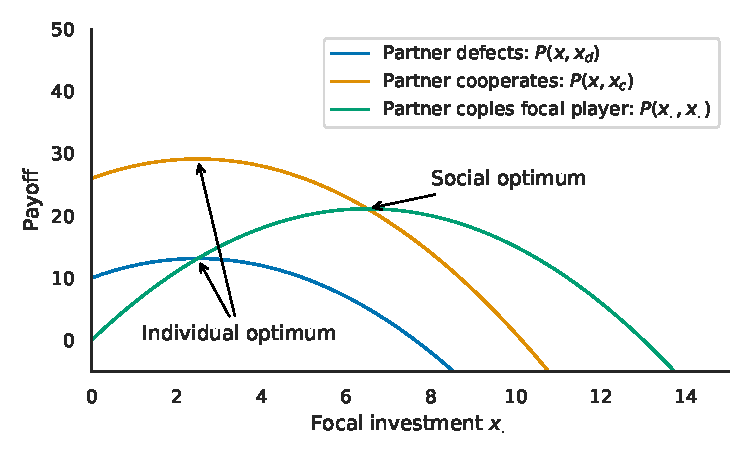
\includegraphics[width=\linewidth]{lions/methods/payoff.pdf}
%     \caption{Variation of the payoff for the focal player according to its partner investment strategy for $n=2$}
%     \label{fig:payoff}
% \end{figure}

% Note: pourquoi social optimum quand P(x, x)? Nécessite une explication qui ne va pas de soi (?).



\subsection{The evolutionary algorithm}\label{sec:evolutionaryalgo}

Each individual has a genome composed of the weights of its two neural networks, which makes a total of 84 genes $g = (g_{1}, \ldots, g_{84})$ with $ g_{i} \in ]-10, 10[$. We consider a population of fixed size $N$. The first generation is composed of $N$ individuals with random genes for the neural network weights, drawn uniformly in $]-1, 1[$. We then use a fitness proportionate evolutionary algorithm to simulate  evolution.  After the $T$ time steps of a generation have taken place, individuals all reproduce and die. A new population of $N$ individuals is built out of the previous generation by sampling randomly among the $N$ parents in proportion to their cumulated payoff, according to a Wright-Fisher process.

A mutation operator is applied on each offspring. Every gene of every offspring has a probability $\mu$ to mutate and a probability $1-\mu$ to stay unchanged. If a gene $g_i$, with value $v_i$, mutates, it has a probability $0.9$ to mutate according a normal distribution and thus reach a new value sampled in $\mathcal{N}(v_i, 0.1)$ and a probability $0.1$ to mutate according to a uniform distribution and thus reach a new value sampled in $\mathcal{U}(]b_{min}, b_{max}[)$.

The evolutionary algorithm is run for $G$ generations.


\begin{table}
    \centering
    \begin{tabular}{clc}
        \hline
        \textbf{Parameter} & \textbf{Description} & \textbf{Value}  \\
        \hline
        \textbf{Environment} & & \\
        $N$ & Population size & $100$ \\
        $d$ & Probability of disappearance of partches, per time step & $1/1\ 000$ \\
        $T$ & Number of timesteps per generation & $1\ 000$ \\
        $c_{m}$ & Cost of moving to another patch & $0$ \\
        $N_T$ & Number of individuals in the local environment & var \\

        \textbf{Payoff } & & \\
        $a$ & Immediate personal benefit of cooperation & $5$ \\
        $b$ & Social benefit of cooperation & $5$ \\
        $\hat{n}$ & Optimal number of individuals per patch & var \\
        $\sigma$ & Tolerance to variations in the number of individuals per patch & var \\
        \textbf{Evolution} & & \\
        $G$ & Number of generations & $1\ 500$ \\
        $\mu$ & Probability of mutation per gene per generation & $0.01$ \\
        \hline

    \end{tabular}
    \caption{Parameters of the simulation}
    \label{tab:parameters}
\end{table}


\section{Results}

\subsection{Cooperation cannot evolve when patches are scarce}

We simulated the evolution of a population of $N_T=100$ individuals for $G=1500$ generations, for different values of the number of resource patches $\omega$, but always in a situation where the optimal number of individuals per patch was $\hat{n}=2$. Cooperation only evolved when patches were more abundant than a threshold (Fig.~\ref{fig:varyingopp}, a). This can be understood as follows. When resource patches are few, precisely when $\omega < \frac{N_T}{\hat{n}}$, individuals have little cooperation opportunities and there is therefore always more individuals per patch than what would be optimal (in this case, the optimal number of individuals per patch is $\hat{n}=2$). As a result, additional individuals joining a patch are more of a nuisance than a benefit, and there is therefore no benefit in trying to attract partners by appearing cooperative.

\begin{figure}[tb]
    \centering
    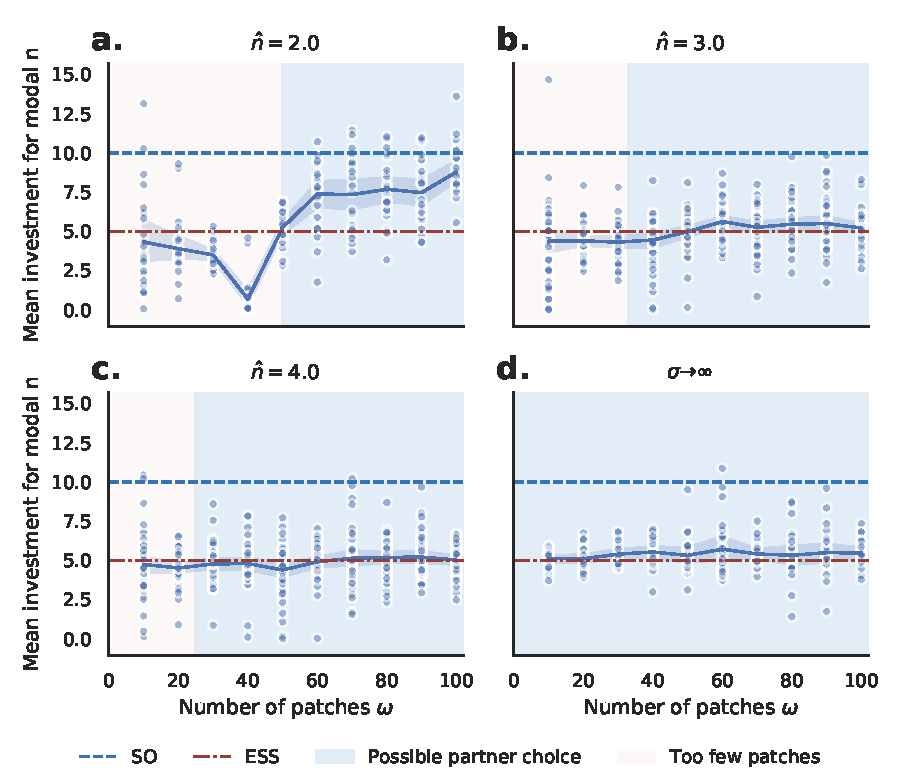
\includegraphics[width=\columnwidth]{lions/results/byprod/varopp_hatn_1.pdf}
    \caption{Mean investment in simulation for different number of opportunities $\omega$ and a fixed population of $N_T=100$ individuals. Results after $1\,500$ generations. \textbf{a.}~When $\hat{n} = 2$ Cooperation evolves when $\omega \geq 50$. \textbf{b-c.}~For $\hat{n} \geq 3$, cooperative behaviours never evolve. \textbf{d.}~When $\sigma \to \infty$, there is no pressure for agent to attract partners and cooperative behaviours never evolve.}
    %\par \small
    %When there is not enough patches to host all the agents in the environment, agents have no outside options. Therefore, they have no better choice than staying with their current partners.
    %If there is enough patches, agents can easily find available opportunities. Therefore, they have plenty of outside options. Partners must invest sufficiently enough to satisfy the agent.

    \label{fig:varyingopp}
\end{figure}


We then simulated the evolution of cooperation in situations where the optimal number of individuals per patch, $\hat{n}$, was larger (Fig. \ref{fig:varyingopp}, b-c). Overall, the outcome was even less favorable to cooperation. This may seem paradoxical but can be understood as a consequence of the law of large numbers. When the number of individuals per patch is large, whether it is greater or less than $\hat{n}$, the effect of each individual on the average quality of her patch is very small anyway. There is therefore little value for an individual to invest in cooperation to try and attract partners.

Finally, we performed the same simulations in the case where the number of individuals per patch is neutral ($\sigma \rightarrow \infty$, Fig. \ref{fig:varyingopp}, d). Cooperation did not evolve either and this can be understood also because there cannot be any benefit in attracting partners when the number of individuals per patch does not matter.

Overall, the evolution of cooperation by partner choice can only take place in the restricted conditions where (i) there is an optimal number of individuals per resource patch, (ii) this optimal number is low, and (ii) the number of resource patches in the environment is large.


\subsection{Cooperation cannot evolve when there are too many partners around}

In a second step, we simulated again the evolution of a population of $N=100$ individuals for $G=1500$ generations in a situation where the optimal number of individuals per patch was $\hat{n}=2$, but this time we held the number of patches constant, $\omega = 20$, while varying the actual number of individuals, $N_T$, present together in the environment.

In this case, cooperation only evolved when the number of individuals in the environment was intermediate. This can be understood as follows. When the number of individuals in the environment, $N_T$, is too close to the number of individuals, $\hat{n}$, that are needed to exploit at least one patch --or even more so when $N_T < \hat{n}$ , then the number of available partners is limiting. As a result, the actual number of cooperation opportunities from which individuals can choose is very low, partner choice is thus a weak force, and the benefit of investing into cooperation is low. On the other hand, when the number of individuals in the environment, $N_T$ is larger than the total number of individuals that can be accomodated on the available patches, that is when $N_T > \hat{n} \omega$, the number of available patches is limiting. In this case we find the result described above (Fig. \ref{fig:gridtol1}, a). The problem is rather that there are always too many individuals on each patch than too few and partner choice is also a weak force. There is, therefore, a range of intermediate population densities, neither too low nor too high, for which cooperation can evolve.

We then performed the same simulations again, but with more patches available in the environment (i.e. for larger $\omega$, Fig. \ref{fig:gridtol1}, b, c). We observed that the range of population densities for which cooperation could evolve was then broader. This can again be understood in the above framework. On one hand, the lower boundary of population density, $N_T \approx \hat{n}$, below which the number of individuals is a limiting factor, is unaffected by the amount of patches available.  On the other hand, the upper boundary of population density, $N_T > \hat{n}\omega$, above which the number of patches is a limiting factor, increases with the amount of patches, $\omega$ . As a result, the width of the range of population densities where partner choice is effective increases.

\begin{figure*}
    \centering
    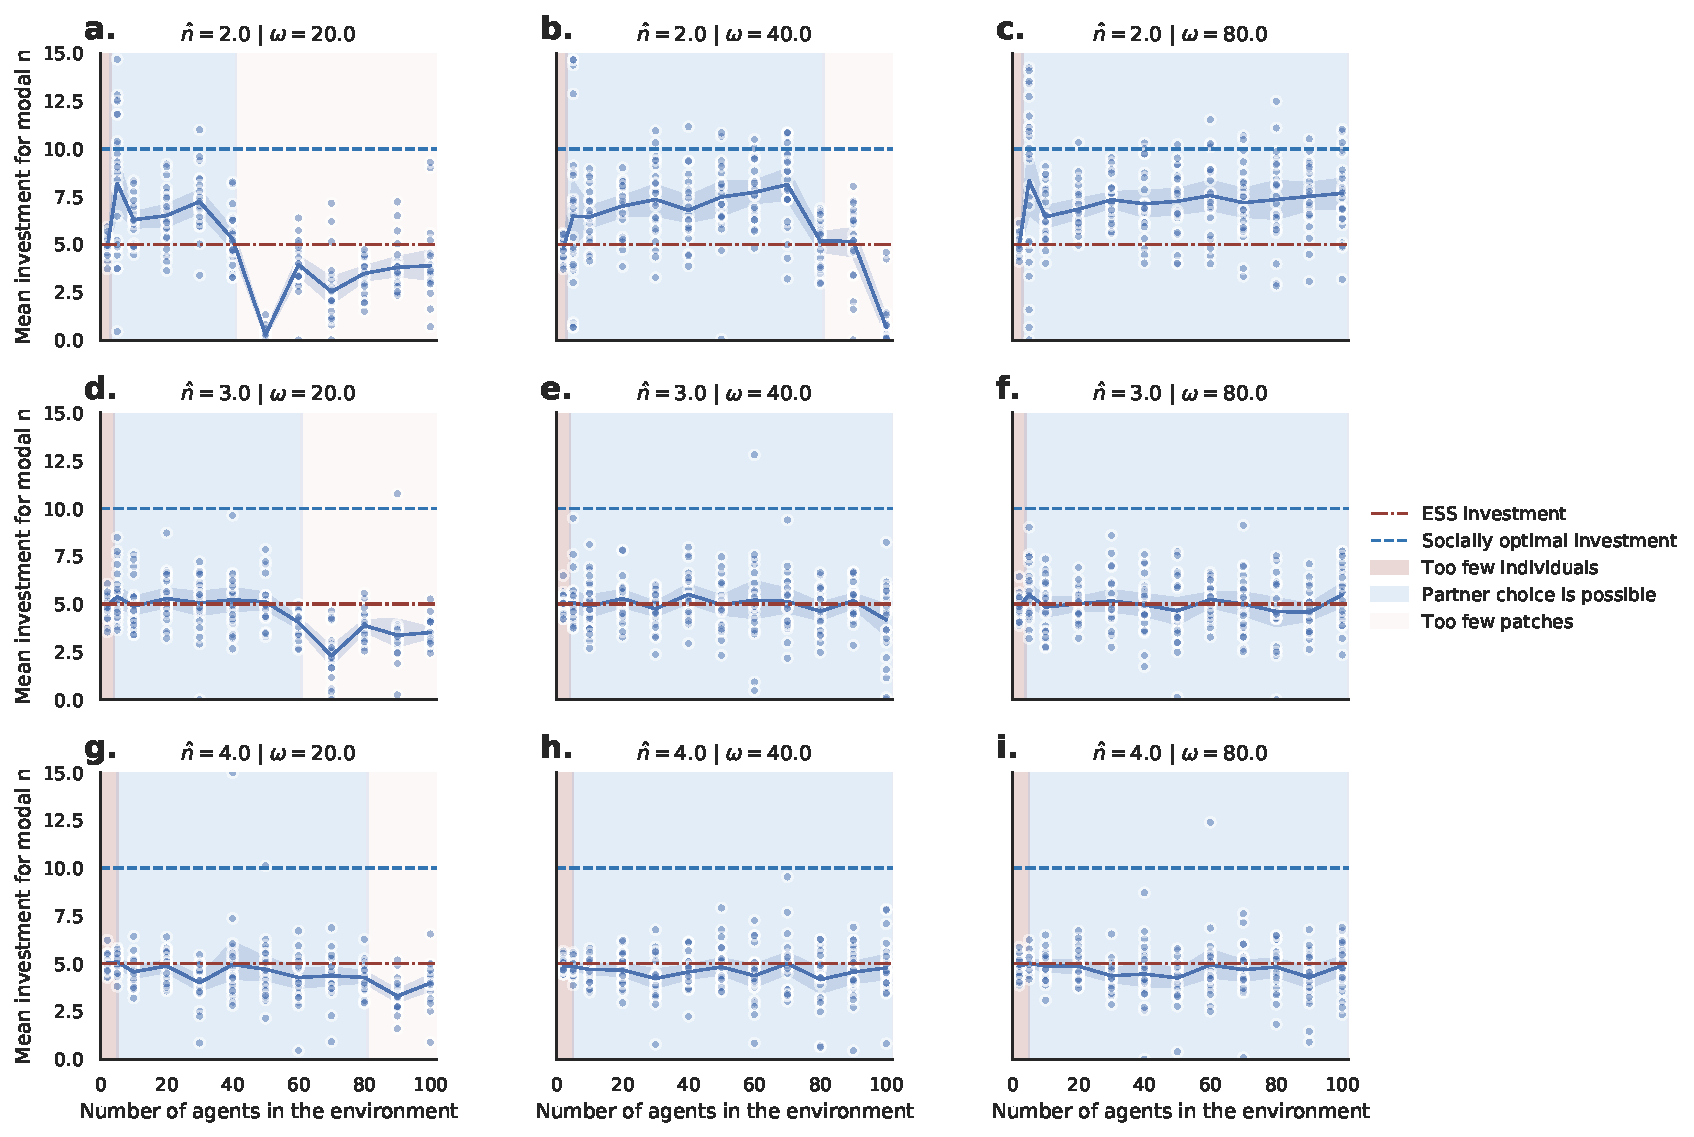
\includegraphics[width=\textwidth]{lions/results/byprod/grid_1.pdf}
    \caption{Effect on the population size in the environment with 20, 40 or 80 patches and an optimal number ofagents $\hat{n} = 2, 3$ and $\sigma = 1$. Agents have a cooperative behaviour for $\hat{n} < N_T < \omega\times \hat{n}$ and for $\hat{n} = 2$.}
    \label{fig:gridtol1}
\end{figure*}

We then performed the same simulations, but this time in situations where the optimal number of individuals per patch, $\hat{n}$, was larger. The outcome was even less favorable to cooperation (Fig.~\ref{fig:gridtol1}, e-p). This is again a consequence of the dilution of the benefit of being a cooperator to attract others, when cooperation takes place in too large groups.

\section{Discussion}

Partner choice can lead to the evolution of cooperation when individuals can compare several opportunities for social interaction and choose the most advantageous. In this article, we have shown that the conditions for this to happen are, however, quite restrictive. They entail  that individuals really have access to a range of social opportunities. Yet, in many cases, social opportunities are very rare because they necessitate the co-occurrence of two things at the same time: (i) at least one available partner, and (ii) an exploitable resource or, more generally, ``something to do'' with that partner. 

Cooperation by partner choice can therefore evolve in two situations. First, it can evolve if a partner constitutes in itself a resource as there is, in this case,  no further requirement for a social opportunity than the need to find a partner. This occurs, for instance, in sexual markets, or in the many instances of interspecific mutualisms where the other individual alone constitutes an opportunity to cooperate. It is therefore logical that partner choice plays an important role in these two types of interactions (refs xx).

Second, it can evolve if individuals are very efficient at extracting opportunities for cooperation from their environment. This is particularly the case in the human species. In the same environment, there are more opportunities for cooperation for human beings than for individuals of most other species. This is a consequence of our skill-intensive strategy that allows us to transform and thereby extract high-value resources from our environment (Kaplan xx). We can thus understand why our cooperation is  related to our cognitive abilities. Having skills that increase the number of opportunities to do useful things also brings with it the possibility of choosing between different opportunities. This puts greater pressure on individuals, who are competing to attract partners on their own opportunity, rather than on another. 

xx revoir cette partie = TODO PAUL = faire la biblio sur les différentes hypothèses sur la relation entre intelligence et coopération (rapidement ; voir mon mail)
There is a large number of hypotheses in the literature on the relationship between intelligence and cooperation and it is often difficult to  sort them out, both in terms of their empirical predictions and in terms of their theoretical plausibility. One particularly prominent theory, the social brain hypothesis, considers that our cognitive abilities are a secondary consequence of selective pressures steming from social life (refs xx). Cooperation is a complex problem to solve that requires the evolution of sophisticated cognitive devices and, so the theory goes, this led to the evolution of intelligence in other domains as well. The social brain hypothesis, however, is based on the premisse that selection to deal with specifically social problems leads to the evolution of intelligence in other domains as well, which is not plausible (refs xx). Another more recent hypothesis considers that causality goes both ways (refs xx west). Intelligence makes cooperation more efficient, which increases the range of situations in which cooperation can evolve, which in turn selects for more intelligence to better benefit from cooperation and so on. The present hypothesis is not in oposition to the latter. It constitutes an additional effect, which specifically concerns reciprocal cooperation --cooperation made to attract partners-- and not other forms of cooperation such as kin altruism or byproduct cooperation. According to our hypothesis, intelligence does not make cooperation more useful, it makes all actions in the world more efficient, and thus leads to greater competition between individuals to attract partners, thereby forcing them to cooperate more.

On the other hand, partner choice cannot lead to the evolution of cooperation when individuals are not very effective in finding cooperation opportunities in their environment. This explains why, in many species, social interactions show no evidence of cooperation beyond immediate self-interest (refs xx). Even when individuals engage in collective actions, for example when they hunt collectively, others have so few outside options anyway that there is no need to seek to draw them into the collective actions. They will come anyway, for want of anything better to do. Even worse than that, as opportunities for cooperation are rare, not only are there always enough partners in each collective action without it being necessary to actively attract them, but in fact the opposite is true. There are always too \textit{many} indviduals participating in each cooperation endeavour. This has been documented for instance in pack hunting in Lions, where Packer showed that lionesses often hunt in groups that are too large compared to what would be optimal (refs xx). In such a case, the average gain per individual in a collective action is reduced and not increased by the participation of others, and there is therefore no selection to attract partners but rather a selection to push them away at the time of sharing.

%The difficulty is that, even in these cases, during the collective action itself, individuals do behave in a coordinated manner for a common goal, as they all wish for the eventual success. Yet, this is no indication that they are cooperating for anything other than their immediate benefit. In many cases, individuals actually live in groups for an independent reason (e.g., to protect against  foreign males in the case of lionnesses) and the most prominent collective actions (e.g. group hunting) are merely unwanted by-products of  group life, occuring because individuals simply have nothing better to do.
